\documentclass[../root]{subfiles}
\graphicspath{{_images/}{../_images/}}

\begin{document}

    \chapter{ Tax-Exempt Lobbying: Corporate Philanthropy as a Tool for Political Influence }

    \begin{shortsummary}
        \begin{itemize}
            \item \authoryear{Bertrand2020} 
            \item \RQ{ Do firms uses corporate social responsibility as a means of political influences? }
            \item \answer{ Construct time-varying pair-specific variable representing political tightness between firms and politicians.
Estimate the effect of this variable on charitable giving toward noprofits associated with politicians, using fixed effect model. }
            \item \result{ Positive effect of political tightness on charitable giving.
The scale of charitable giving is 2.5 times larger than political acticon committee (PAC) contributions. }
        \end{itemize}
    \end{shortsummary}

    \section{RQ}\label{rq}

    \begin{itemize}
    
    \item
      政治家は様々なルートによってロビー活動を受ける

      \begin{itemize}
      
      \item
        選挙運動への寄付、天下り先の提示など
      \end{itemize}
    \item
      過去の研究の多くは、選挙運動への寄付とロビー活動の関係に焦点を当てていた

      \begin{itemize}
      
      \item
        データが観察しやすいが、ロビー活動の全体の規模に対して小さいという批判がある
      \item
        ロビー活動の規模と範囲を理解するために、他のルートで政治に影響を与える方法があるのかを調べる必要がある
      \end{itemize}
    \item
      この研究は、\textbf{アメリカ政治において、企業のフィランソロピー活動はロビー活動の道具として利用していて、その規模が他のチャンネルと比べて規模が大きいことを示す}

      \begin{itemize}
      
      \item
        フィランソロピー活動が政治の道具として使える理由として、有権者が政治家が関与する慈善団体の功績を観察しやすいので、政治家の功績として投票者にアピールしやすいことが考えられる(credit-claiming)
      \item
        見返り政治の結果として投票者が考える最適な政治を歪めてしまうので、厚生の損失が生じる(この手のロビー活動は有権者や株主に見えづらいという問題点があり、慈善団体への最適配分からも乖離する可能性がある)
      \end{itemize}
    \end{itemize}

    \section{分析アイデア}\label{ux5206ux6790ux30a2ux30a4ux30c7ux30a2}

    \begin{figure}
    \centering
    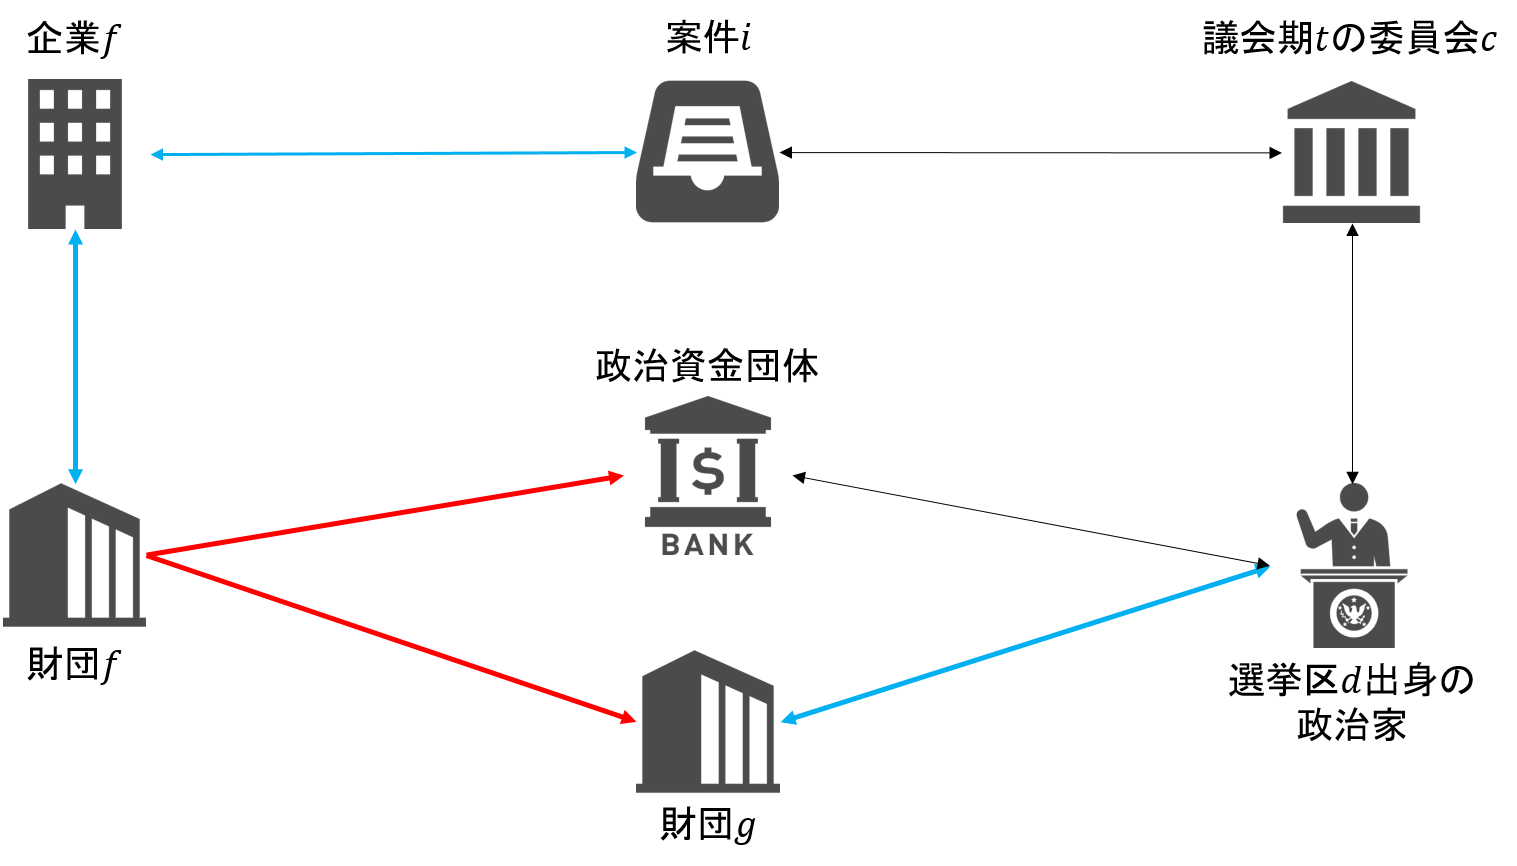
\includegraphics[width = .8\linewidth]{0911kato/92577460-a0e40a80-f2c5-11ea-8ecb-de283c56fa5b.png}
    \caption{ストーリー}
    \end{figure}

    \begin{itemize}
    
    \item
      \textbf{仮説となるストーリー}:第\(t\)議会で案件\(i\)について議論される委員会\(c\)が開催される。企業\(f\)がその案件を自身の収益に重大な影響を与えると考えているとき、その委員会に所属する選挙区\(d\)出身の政治家に対して非営利団体\(g\)への寄付を通じてロビー活動を行う。
    \item
      Identification source: (a) 委員会のメンバーが議会期で入れ替わる、(b) 企業が関心のある案件が議会期に応じて変化する(variation across \(t\))

      \begin{itemize}
      
      \item
        メインの説明変数はtime varying pair-specific (\(f \times d \times t\)) な変数となる
      \item
        パネルデータを構築して固定効果モデルで因果効果を識別する
      \end{itemize}
    \item
      企業\(f\)が関心のある案件の特定化

      \begin{itemize}
      
      \item
        連邦選挙委員会が出元の情報をまとめている非営利組織The Center of Responsive Politics (CRP)が、企業\(f\)が特定の案件\(i\)へのロビー活動の費用を公開している。これを用いて、どの案件に関心があるかを特定化する
      \end{itemize}
    \item
      政治家と非営利団体\(g\)をリンクさせるために二つの方法を用いる

      \begin{enumerate}
      \def\labelenumi{\arabic{enumi}.}
      
      \item
        Geographical link: 非営利団体の所在地が選挙区\(d\)内にあるかどうか(地元の非営利活動に対して率先的である事実でこの方法の妥当性を保証している)
      \item
        Direct personal link: 委員会に所属する政治家は自身の財務情報開示する法律がある。その法律によって、所属する非営利団体でのポジション(たいてい取締役会)を開示する必要があるので、非営利団体の名前でリンクすることができる

        \begin{itemize}
        
        \item
          ただし、その開示情報はポジションに就いていた期間が明記されていないので、このリンクはtime-invariantである
        \end{itemize}
      \end{enumerate}
    \end{itemize}

    \subsection{データ}\label{ux30c7ux30fcux30bf}

    \begin{itemize}
    
    \item
      複数のデータベースをつなぎ合わせてパネルデータを構築する
    \end{itemize}

    \begin{table}
          \centering
          \caption{Data Source}
          \begin{adjustbox}{max width=\textwidth}
          \begin{tabular}{cc}
            \hline
            データベース & 含まれる情報 \\
            \hline\hline
            FoundationSearch &
            財団\(f\)の名前、財団の寄付に関する情報(団体名、所在地、金額、寄付のタイプ)\\
            Form990 &
            財団の財務情報(財団の基礎情報、資産、\$4000以上の拠出をした非営利組織の列挙)\\
            CRP & 
            政治家のPFDデータ、企業のロビー活動(PAC contributionを含む) \\
            Charles Stewart III's web site & 委員会のメンバー \\
            Poole and Rosenthal's web site & 委員会のメンバー \\
            voteview.com & 委員会のメンバー \\
            \hline
          \end{tabular}
        \end{adjustbox}
        \end{table}

    \begin{itemize}
    
    \item
      財団\(f\)の名前にS\&P500もしくはFortune500に属する企業の名前が入る324財団を用いる
    \item
      データ期間は1998年から2014年(第105回議会-第113回議会)
    \end{itemize}

    \subsection{主な発見}\label{ux4e3bux306aux767aux898b}

    \begin{enumerate}
    \def\labelenumi{\arabic{enumi}.}
    
    \item
      企業の寄付とPAC(政治家の政治資金団体で企業からの資金を集めてそれを献金する)への提供額が正の相関

      \begin{itemize}
      
      \item
        政治への影響が企業寄付のモチベーションとなっているかもしれない
      \end{itemize}
    \item
      政治家との関わりが強いほど、企業が政治家の関わる慈善団体への寄付額を増やす

      \begin{itemize}
      
      \item
        とくに、政治家が慈善団体の取締役会に名を連ねていると、受け取る寄付額は4倍になる
      \end{itemize}
    \item
      一般的なモデルと仮定のもとで、企業のCSR活動のうち6.3\%が政治的な寄付であった

      \begin{itemize}
      
      \item
        2014年のCSRの規模が1800万ドルなので、113万ドルが政治的な寄付に使われた。この額はその年のPACへの資金提供規模の2倍に相当し、ロビー活動費用の35\%に相当する.
      \end{itemize}
    \end{enumerate}

    \section{Geographical Link Analysis}\label{geographical-link-analysis}

    政治家と非営利団体のつながりをgeographical linkを用いて分析する。

    \begin{equation}
    \ln(1 + Contributions_{fdt}) = \beta_0 + \beta_1 \ln(1 + IssuesCovered_{fdt}) + \delta_{fd} + \gamma_{dt} + \epsilon_{fdt}
    \end{equation}

    \begin{itemize}
    
    \item
      \(Contributions_{fdt}\): 企業の寄付

      \begin{enumerate}
      \def\labelenumi{\arabic{enumi}.}
      
      \item
        議会期\(t\)における選挙区\(d\)出身の政治家への企業\(f\)のPAC contributions(政治家の政治資金団体)
      \item
        議会期\(t\)における選挙区\(d\)内に所在する非営利団体\(g\)への企業\(f\)のCSR contributions
      \end{enumerate}
    \item
      \(IssuesCovered_{fdt} = \sum_c \sum_i l_{fit} x_{ic} Membership_{cdt}\)

      \begin{itemize}
      
      \item
        \(l_{fit} = 1\): 議会期\(t\)における企業\(f\)のロビー活動に最も多く費やした案件\(i\)である
      \item
        \(x_{ic} = 1\): 委員会\(c\)で審議されている案件\(i\)である
      \item
        \(Membership_{cdt} = 1\): 議会期\(t\)において選挙区\(d\)出身の政治家が委員会\(c\)に参加している
      \end{itemize}
    \item
      \(\delta_{fd}\): 財団\(f\) \(\times\) 選挙区\(d\)の固定効果

      \begin{itemize}
      
      \item
        企業\(f\)のpreferences for local charitiesの効果を排除する
      \end{itemize}
    \item
      \(\gamma_{dt}\): 選挙区\(d\) \(\times\) 議会期\(t\)の固定効果

      \begin{itemize}
      
      \item
        特定の選挙区の重要性が増し、そこ出身の政治家が地元のビジネスに関連する委員会に参加する可能性が高くなる。これによる寄付の効果を排除する。
      \item
        (コメント)正直この重要性はわからない
      \end{itemize}
    \end{itemize}

    \subsection{記述統計1}\label{ux8a18ux8ff0ux7d71ux8a081}

    \begin{figure}
    \centering
    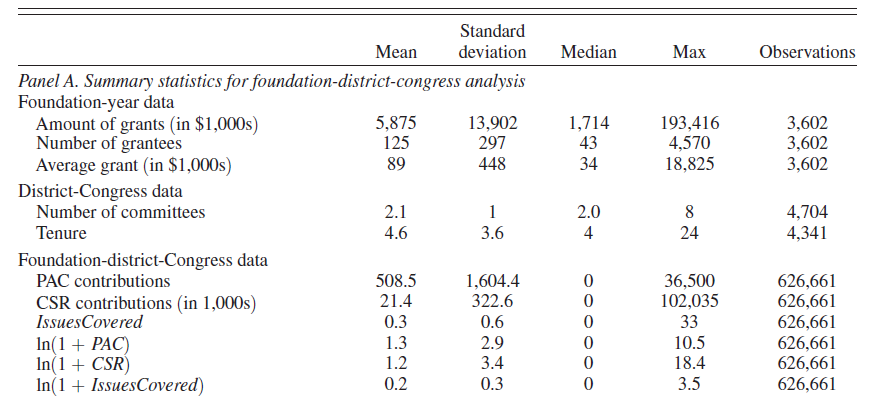
\includegraphics[width = .8\linewidth]{0911kato/92602660-64c2a100-f2e9-11ea-8ec8-7535de579a5d.png}
    \caption{記述統計}
    \end{figure}

    \subsection{結果1: PAC contributionsとCSR contributionsの関係}\label{ux7d50ux679c1-pac-contributionsux3068csr-contributionsux306eux95a2ux4fc2}

    \begin{figure}
    \centering
    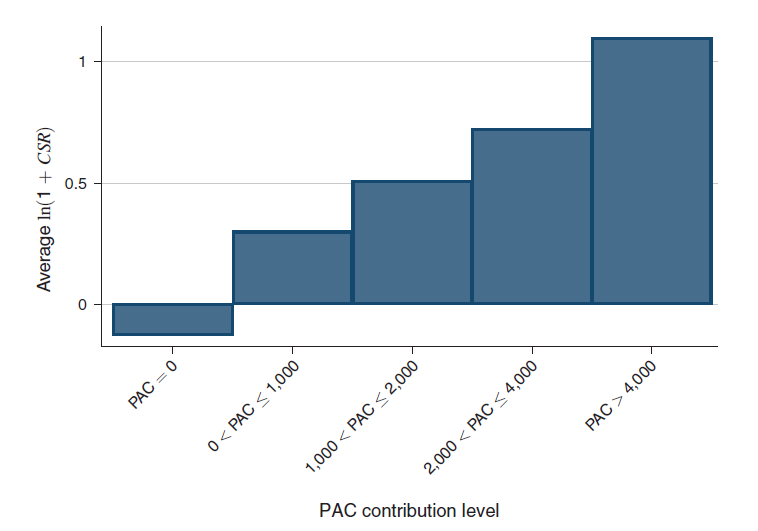
\includegraphics[width = .8\linewidth]{0911kato/92603528-5f198b00-f2ea-11ea-848f-dbf2ca9d349b.png}
    \caption{PAC and CSR Contributions}
    \end{figure}

    \begin{itemize}
    
    \item
      PAC contributionsとCSR contributionsは正の相関をしていることがわかる

      \begin{itemize}
      
      \item
        \(\ln(1 + CSR)\)を財団\(f\) \(\times\) 議会期\(t\)の固定効果で回帰して、その残差の平均値をプロットしたもの
      \item
        \(\delta_{fd}\)と\(\gamma_{dt}\)をコントロールしても正の相関は確認できる
      \end{itemize}
    \end{itemize}

    \subsection{結果2: Issues Coveredとの関係}\label{ux7d50ux679c2-issues-coveredux3068ux306eux95a2ux4fc2}

    \begin{figure}
    \centering
    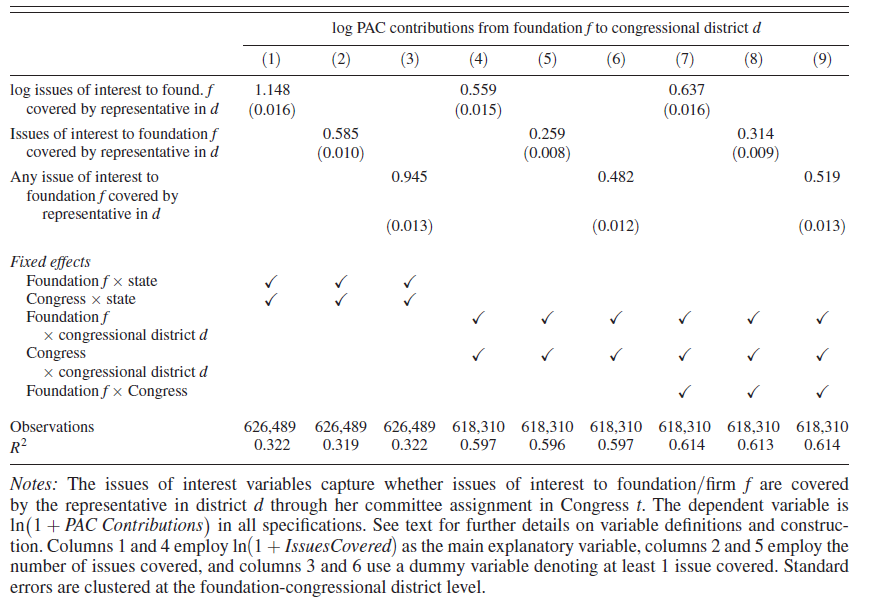
\includegraphics[width = .8\linewidth]{0911kato/92604588-a2c0c480-f2eb-11ea-8dd4-69d392ca2875.png}
    \caption{PAC Contributions and Issues Covered}
    \end{figure}

    \begin{itemize}
    
    \item
      Column 1, 4, and 7はIssues Coveredに対するPACの弾性値を示す

      \begin{itemize}
      
      \item
        ある政治家が抱える企業の関心のある案件が1\%増えたら、PAC contributionsは0.56-1.15\%増える
      \item
        今後はcolumn 7の結果を用いる。弾性値は0.637
      \end{itemize}
    \end{itemize}

    \begin{figure}
    \centering
    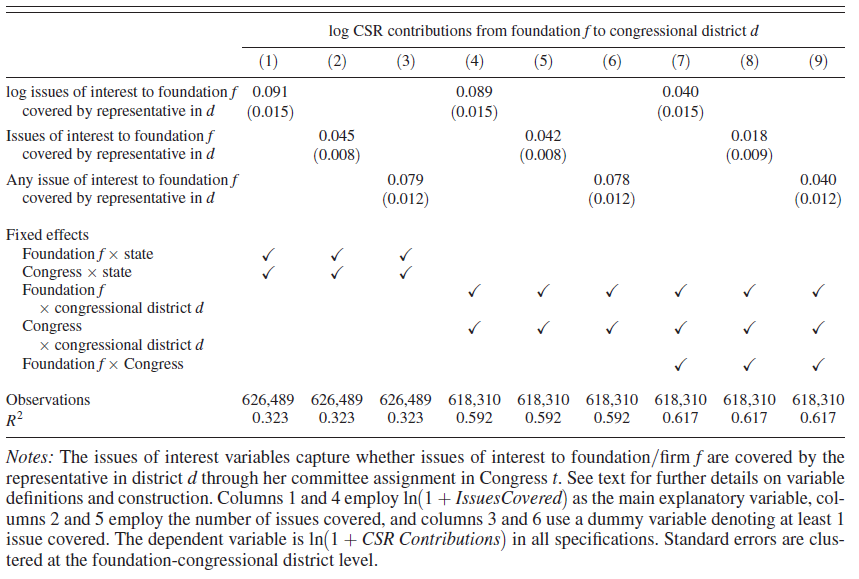
\includegraphics[width = .8\linewidth]{0911kato/92605313-8a9d7500-f2ec-11ea-9695-088e163dd4c6.png}
    \caption{CSR contributions and Issues Covered}
    \end{figure}

    \begin{itemize}
    
    \item
      Column 1, 4, and 7はIssues Coveredに関するCSRの弾性値を示し、その範囲は0.040-0.091である

      \begin{itemize}
      
      \item
        今後はcolumn 7の結果を用いる。弾性値は0.040
      \item
        非営利団体の種類ごとに推計した結果、教育、公益、国際、宗教やヒューマンサービスに関する組織の方が弾力的である
      \end{itemize}
    \item
      以下のロバスト分析をしても結果に変化はない

      \begin{enumerate}
      \def\labelenumi{\arabic{enumi}.}
      
      \item
        extensive margin
      \item
        二次項を加えた非線形モデル
      \item
        対数化しない回帰分析
      \item
        対数化するときに足す値を変更
      \end{enumerate}
    \item
      Remarks

      \begin{itemize}
      
      \item
        サンプルピリオドで最もロビー活動に費やした案件で\(IssuesCovered\)を作成した結果、弾性値は小さくなるが統計的に有意である(この場合、\(IssuesCovered\)のvariationは委員会の入れ替わりのみである)
      \item
        委員会に参加している政治家ではなく、委員会の委員長やその他重要な役職についている政治家に焦点を当てると、弾性値は30-40\%増加する
      \end{itemize}
    \end{itemize}

    \subsection{結果3: Exit House Memberの効果}\label{ux7d50ux679c3-exit-house-memberux306eux52b9ux679c}

    \begin{figure}
    \centering
    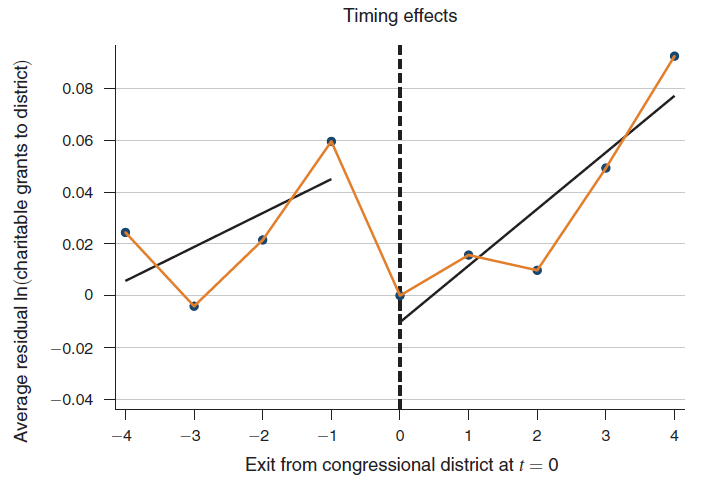
\includegraphics[width = .8\linewidth]{0911kato/92611263-93457980-f2f3-11ea-941c-8eb0d34996b9.png}
    \caption{CSR Contributions and House Member Exits}
    \end{figure}

    \begin{figure}
    \centering
    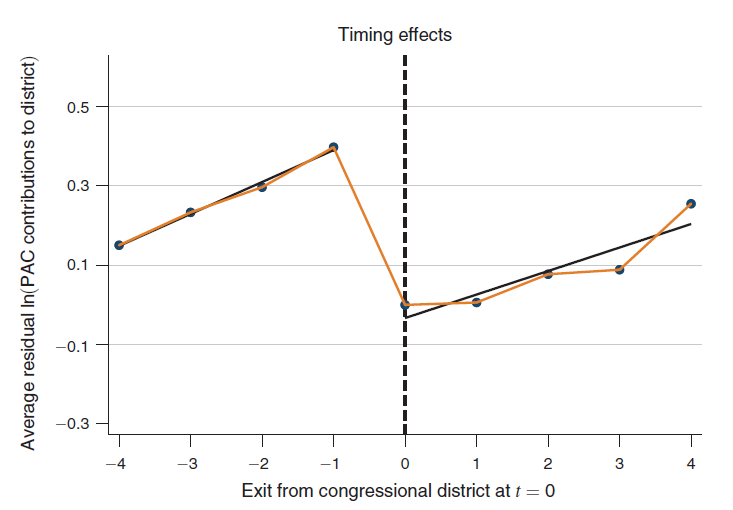
\includegraphics[width = .8\linewidth]{0911kato/92611372-ae17ee00-f2f3-11ea-99c1-4a91a7a0ea07.png}
    \caption{PAC Contributions and House Member Exits}
    \end{figure}

    \begin{itemize}
    
    \item
      \(\ln(1 + Contributions_{fdt})\)を\(\delta_{fd}\)と\(\gamma_{dt}\)で回帰分析した残差の平均値を退出タイミングを中心に各ピリオドごとにプロット

      \begin{itemize}
      
      \item
        下院議会の退出時に選挙区\(d\)への寄付金が減少し、新たに入り直し、その地位を高めることで寄付金が上昇する
      \end{itemize}
    \end{itemize}

    \section{Direct Personal Link Analysis}\label{direct-personal-link-analysis}

    政治家の財務情報を用いて非営利団体と直接的にリンクさせて分析する。このとき、選挙区\(d\)出身の政治家\(=\)非営利団体\(g\)である。

    \begin{equation}
    AnyGiving_{fgt} = \beta \times AnyRelevant_{fgt} + \omega_{fg} + v_t + \epsilon_{fgt}
    \end{equation}

    \begin{itemize}
    
    \item
      \(AnyGiving_{fgt} = 1\): 議会期\(t\)において企業の財団\(f\)が政治家が取締役会に所属する非営利団体\(g\)に寄付した
    \item
      \(AnyRelevant_{fgt} = 1\): 議会期\(t\)において企業\(f\)のロビー活動と政治家(が所属する非営利団体\(g\))の関与が被る案件がある

      \begin{itemize}
      
      \item
        \(Relevant(\#issues)\): 被っている案件の数
      \item
        \(Relevant(\#Congressmen)\): 政治家(が所属する非営利団体\(g\))が、企業がロビー活動している案件を審議する委員会に参加している数
      \item
        \(Relevant(\#Congressmen-issue pairs)\): 政治家の関与と企業のロビー活動が被っている案件と委員会のペアの数
      \end{itemize}
    \end{itemize}

    \subsection{記述統計2}\label{ux8a18ux8ff0ux7d71ux8a082}

    \begin{figure}
    \centering
    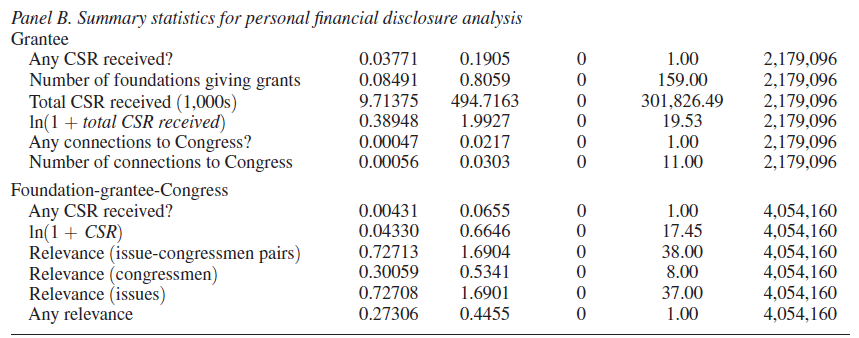
\includegraphics[width = .8\linewidth]{0911kato/92614392-f389ea80-f2f6-11ea-8b28-0cfd40735f4a.png}
    \caption{Descriptive Statistics (Continued)}
    \end{figure}

    \subsection{結果: CSR contributions}\label{ux7d50ux679c-csr-contributions}

    \begin{figure}
    \centering
    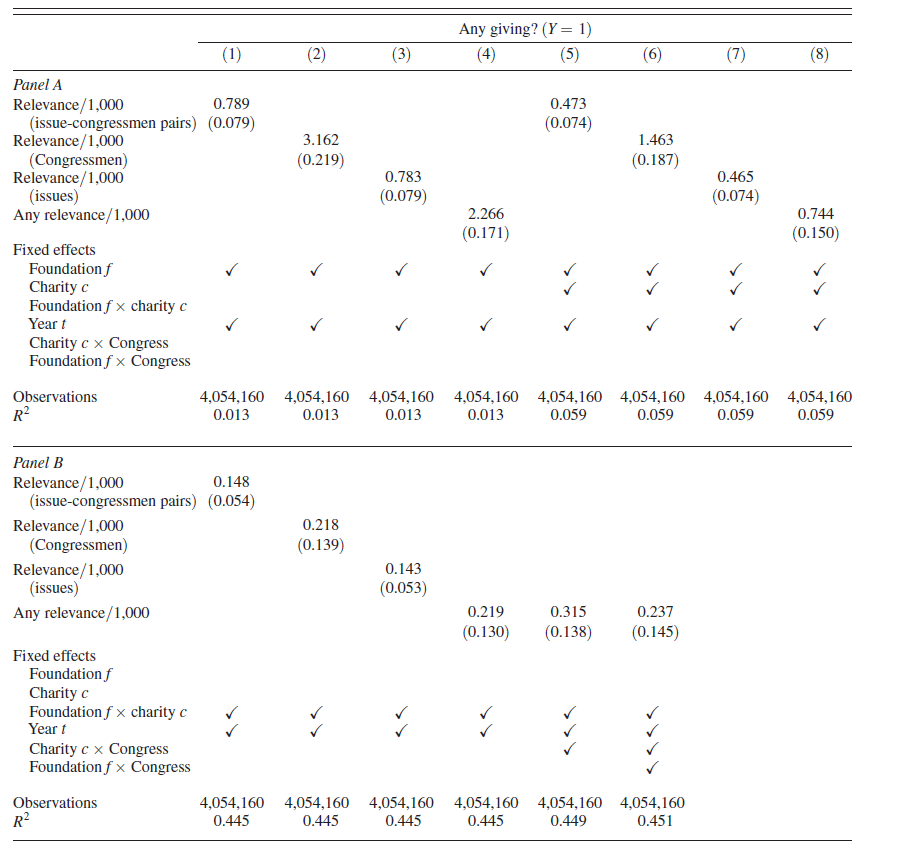
\includegraphics[width = .8\linewidth]{0911kato/92614724-57141800-f2f7-11ea-8d26-69fcdf3894a7.png}
    \caption{CSR Contributions to Relevant Charities}
    \end{figure}

    \begin{itemize}
    
    \item
      Panel Aのcolumn 3: ロビー活動の案件に非営利団体が関与しているとき、寄付する確率が0.00078増加する

      \begin{itemize}
      
      \item
        寄付確率は0.0043なので、18\%上昇している
      \item
        Panel Aのcolumn 7より寄付確率の上昇は10\%、Panel Bのcolun 3より寄付確率の上昇は3.5\%になる
      \end{itemize}
    \end{itemize}

    \section{Quantifying Politically-Motivated CSR Scale}\label{quantifying-politically-motivated-csr-scale}

    CSRのデータは純粋なCSRと政治的なモチベーションのCSRを識別することができない。
    そこで、理論的なフレームワークを組んで、弾性値の推定値から政治的なモチベーションのCSRの規模を推定する。

    \subsection{Model}\label{model}

    \begin{itemize}
    
    \item
      CSR contributionsとPAC contributionsの定義

      \begin{itemize}
      
      \item
        \(C\): 政治的なモチベーションのCSR規模(非課税による価格低下\(q < 1\))
      \item
        \(\tilde{C}\): 非政治的なモチベーションのCSR規模
      \item
        \(P\): PAC contributions
      \end{itemize}
    \item
      \(\tau = h(A, C, P)\): 企業の関心のある政策の生産関数

      \begin{itemize}
      
      \item
        \(A\): 企業の関心のある政策を審議する委員会へのアサイメントであり、\(P\)と\(C\)の生産性を高める
      \end{itemize}
    \end{itemize}

    企業の最適化問題

    \begin{equation}
    \max_{C,P} h(A, C, P) - qC - P
    \end{equation}

    \subsection{Assumptions and Claim}\label{assumptions-and-claim}

    \textbf{Assumptions}

    \begin{enumerate}
    \def\labelenumi{\arabic{enumi}.}
    
    \item
      パラメータ\(A\)はPACとCSRの生産性を同程度高める(Hicks-neutral productivity shock)

      \begin{itemize}
      
      \item
        これを正当化する説明なし
      \end{itemize}
    \item
      PAC contributions \(P\)は完全に政治的なモチベーションに起因する
    \item
      非政治的なモチベーションのCSRとパラメータ\(A\)は直行する(\(\tilde{C}\)は完全に政治的なモチベーションでない): \((d\tilde{C}/\tilde{C})/(dA/A) = 0\)
    \end{enumerate}

    \textbf{Claim}

    If \(h(A, C, P) = Ag(f(C, P))\) where \(g(\cdot)\) is an increasing and concave function and \(f(\cdot)\) is increasing, quasi-convex, and homogeneous of degree 1, then the elasticity of \(C\) and \(P\) w.r.t. \(A\) is identical:

    \begin{equation}
    \frac{dC}{C}/\frac{dA}{A} = \frac{dP}{P}/\frac{dA}{A}
    \end{equation}

    \subsection{Exercise Result}\label{exercise-result}

    三つの仮定より、PACの弾性値を用いて、以下を得る

    \begin{equation}
    \frac{dC}{C}/\frac{dA}{A} = \frac{dP}{P}/\frac{dA}{A} = 0.637
    \end{equation}

    また、CSR全体の弾性値は以下のようになる

    \begin{equation}
    \frac{dC}{C + \tilde{C}}/\frac{dA}{A} = \frac{dP}{P}/\frac{dA}{A} = 0.040
    \end{equation}

    したがって、

    \begin{equation} 
    (\frac{dC}{C + \tilde{C}}/\frac{dA}{A})/(\frac{dC}{C}/\frac{dA}{A}) = \frac{dC}{C + \tilde{C}}/\frac{dC}{C} = 0.063
    \end{equation}

    よって、\(C/(C + \tilde{C}) = 6.3\%\)を得る。
    2014年におけるCSR規模は180億ドルなので、そのうち政治的なモチベーションのCSR規模は11.7億ドルである。
    2014年におけるPAC規模は4.64億ドルであることを考えれば、政治的なモチベーションのCSR規模はPAC規模の2.5倍となる

    \section{Conclusions}\label{conclusions}

    \begin{quote}
    In documenting the relationship between political interests and private corporate charitable giving, we highlight the ambiguous social welfare consequences of firms'corporate social responsibility. While this point has been noted previously, we are among the first to provide robust empirical evidence speaking to such concerns.
    \end{quote}

    \biblio

\end{document}